% !TeX spellcheck = en_GB
       \documentclass[aspectratio=169]{beamer}
%	\usetheme{warsaw}
            \usepackage{setspace}
            \usepackage{graphicx} %draft option suppresses graphics dvi display
            \newcommand{\Prob}{\operatorname{Prob}}
            \clubpenalty 5000
            \widowpenalty 5000
            \renewcommand{\baselinestretch}{1.23}
            \usepackage{amsmath}
            \usepackage{amsthm}
            \usepackage{amsfonts}
            \usepackage{amssymb}
            \usepackage{bbm}
            \usepackage{cancel}
            \usepackage{soul}
	 \newcommand{\E}{\mathbb{E}}
	 \newcommand{\pd}[2]{\frac{\partial#1}{\partial#2}}
	\newcommand{\bi}{\begin{itemize}}
	\newcommand{\ei}{\end{itemize}}
	\newcommand{\Die}{\mathsf{D}}
	\newcommand{\Live}{\cancel{\Die}}

\author{Matthew N. White}

\title[add]{ECOG 315 / ECON 181, Summer 2025 \\ Advanced Research Methods and Statistical Programming \\ Week 1 Lecture Slides}

\institute[HU]{Howard University}

\date{May 30, 2025}

\begin{document}

% ========== Title slide =================
\begin{frame}
\maketitle
\end{frame}

% ======== Personal introductions =========

\begin{frame}
\frametitle{Who Are These Guys? Matt White}
\begin{itemize}
	\item Instructor of record: Matthew N. White (Matt)
	
	\item Email: \texttt{mnwhite@gmail.com}; ~ Cell: (603) 566 0413
	
	\item I will be here \textbf{most} weeks; others will be here \textbf{sometimes}
	
	\item Previously at University of Delaware, now with Econ-ARK
	
	\item Primary interests: health economics, heterogeneous agents macro
\end{itemize}
\end{frame}

\begin{frame}
\frametitle{Who Are These Guys? Matt White}
\centering
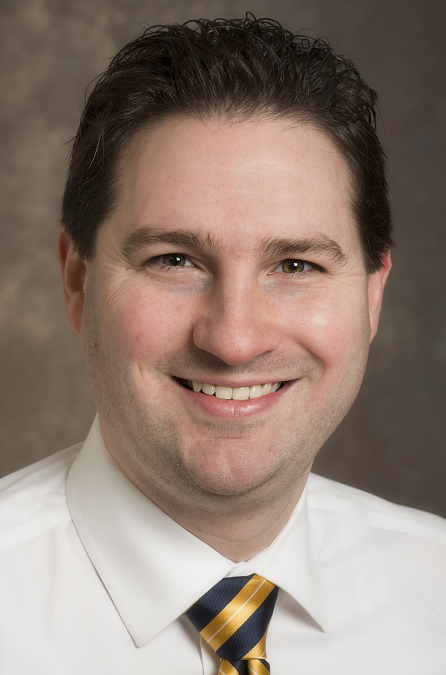
\includegraphics[scale=0.4]{../../media/matt-white.png}
\end{frame}

\begin{frame}
\frametitle{Who Are These Guys? Chris Carroll}
\begin{itemize}
	\item Most senior instructor: Christopher D. Carroll (Chris)
	
	\item Email: \texttt{ccarroll@jhu.edu}
	
	\item Professor at Johns Hopkins economics department
	
	\item World expert in consumption-saving theory and empirics
	
	\item Has advised many PhDs, taught research skills course
\end{itemize}
\end{frame}

\begin{frame}
\frametitle{Who Are These Guys? Chris Carroll}
\centering
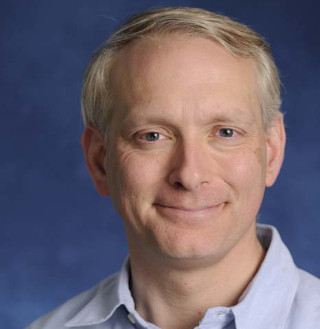
\includegraphics[scale=2.0]{../../media/chris-carroll.jpg}
\end{frame}

\begin{frame}
\frametitle{Who Are These Guys? Alan Lujan}
\begin{itemize}
	\item Content-producing instructor: Alan E. Lujan-Solis (Alan)
	
	\item Email: \texttt{alujan@jhu.edu}
	
	\item Program coordinator and lecturer at JHU Advanced Academic Programs
	
	\item Primary interests: computational methods for economics
	
	\item Will make and share \textbf{asynchronous} Zoom videos
\end{itemize}
\end{frame}

\begin{frame}
\frametitle{Who Are These Guys? Alan Lujan}
\centering

\includegraphics[scale=0.5]{../../media/alan-lujan.png}
\end{frame}

\begin{frame}
\frametitle{Who Are These Guys? Econ-ARK}
\begin{itemize}
	\item All of your instructors work for or with Econ-ARK
	
	\item Non-profit org that makes open source software for economists
	
	\item And tools/structures for archiving research projects
	
	\item Website: \texttt{http://www.econ-ark.org}
	
	\item We didn't expect to be teaching the course, please bear with us!
\end{itemize}

\centering

\includegraphics[scale=0.5]{../../media/econ-ark-logo.png}
\end{frame}

% ======== Website & communication =========

\begin{frame}
\frametitle{Course Communication Channels}
\begin{itemize}
	\item We don't have access to Canvas or class list (yet)
	
	\item GitHub repository: \texttt{https://github.com/econ-ark/aeasp.2025}
	
	\item The repo is ``live'' and edited frequently; you will submit via pull requests
	
	\item <2->If you have questions, please email us, especially Matt
	
	\item <2->If it's something of concern to others, open an issue on GitHub
	
	\item <2->Each team will meet weekly with their advisor, scheduled independently
	
	\item <3->Matt and Alan use Discord; do you want to use Discord for the course?
\end{itemize}
\end{frame}

% ======== How to be an economist =========

\begin{frame}
\frametitle{Big Picture: How to Be an Economist}
\begin{itemize}
	\item You will learn a \textbf{lot} in an economics PhD program
	
	\item Lots of economics, lots of math, lots of econometrics
	
	\item <2->How to \textbf{do} research: asking question, lit review, forming strategy, iterating
	
	\item <2->How to \textbf{communicate}: academic writing, presentations/slides, selling yourself
	
	\item <3->There are tools to help you with those things; often not explicitly taught
	
	\item <3->Being familiar with the tools of the trade is part of being an academic / economist
\end{itemize}
\end{frame}

% ======== Course overview =========

\begin{frame}
\frametitle{What Are We Doing Here? Course Overview}
\begin{itemize}
	\item We are going to help you learn to be an economist
	
	\item In lectures: teaching you about tools used in research and collaboration
	
	\item In lectures: advice for executing research steps and applying those tools
	
	\item <2->In lectures: presenting your research progress and getting feedback
	
	\item <3->Asynchronous Zoom: specific applied econometrics and computational methods
	
	\item <4->Adviser meetings: ongoing personal discussions of your research progress
	
	\item <5->Grading: qualitative hand-waving
\end{itemize}
\end{frame}

\begin{frame}
\frametitle{The Platinum Rule}
\begin{itemize}
	\item Google is your friend; the internet is full of lies, but use it anyway
	
	\item Someone else almost surely had the same Q you did, and got an answer
	
	\item <2->We will also show you how to \textbf{responsibly} use AI in your work
	
	\item <3->WRONG: ``Please write me a 1000 word essay about X, and provide citations.''
	
	\item <3->RIGHT: ``I think these two paragraphs are too wordy and repetitive. Please help me shorten and clarify them.''
\end{itemize}
\end{frame}

% ======== Today's agenda =========

\begin{frame}
\frametitle{Agenda for Week 1}
\begin{itemize}
	\item \st{Personal and course introductions}
	
	\item Installing Anaconda distribution of Python
	
	\item Setting up GitHub account and GitHub Desktop
	
	\item Interacting with course repo via GitHub
	
	\item Basics of \texttt{conda} environments
	
	\item Basics of Python / IDEs / Jupyter notebooks
\end{itemize}
\end{frame}

% ======== Python: why? =========

\begin{frame}
\frametitle{Why Python?}
\centering
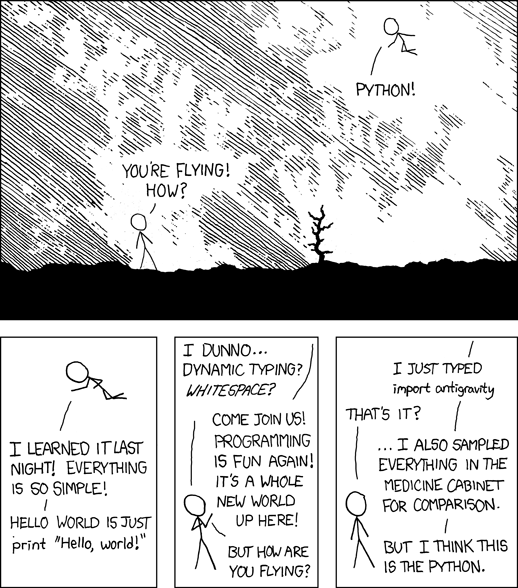
\includegraphics[scale=0.35]{../../media/xkcdpython.png}
\end{frame}

\begin{frame}
\frametitle{Why Python?}
\begin{itemize}
	\item High level language: closer to human language than machine code
	
	\item Well documented and supported: \textbf{many} packages available via PyPI
	
	\item <2->Widely used in scientific computing
	
	\item <2->Completely free and open source
	
	\item <3->Easy to program and run native Python code; human time is valuable
	
	\item <3->Easy to extend and link to other languages: acceleration via \texttt{jit}
	
	\item <4->Not the best at anything, but good enough at everything
\end{itemize}
\end{frame}

% ======== Installing Anaconda =========

\begin{frame}
\frametitle{Anaconda Distribution}
\begin{itemize}
	\item Python comes in \textbf{distributions}: specific implementations with packages
	
	\item Anaconda: widely used distribution for scientific computing
	
	\item <2->Automatically includes all of the most commonly used packages for scientific work
	
	\item <2->Has its own virtual environment and package manager, \texttt{conda}
	
	\item <3->Also comes with a pretty nice interactive development environment (IDE), Spyder
	
	\item <3->Spyder is set up for IPython: better graphical presentation
\end{itemize}
\end{frame}

\begin{frame}
\frametitle{Installing Anaconda}
\begin{itemize}
	\item Go to \texttt{https://www.anaconda.com/download}
	
	\item Submit your email or click ``skip registration''
	
	\item Select the distribution installer for your OS
	
	\item You probably want the graphical installer if it's an option
	
	\item Download it, then install Anaconda; this will take a bit
\end{itemize}
\end{frame}

% ======== Version control and collaboration: git =========

\begin{frame}
\frametitle{Collaboration and Version Control with \texttt{git}}
\begin{itemize}
	\item You have done group work; probably shared docs by email or Dropbox
	
	\item Academic research is a really big group project: so many files
	
	\item <2->Multiple people working on same file at the same time: oh no!
	
	\item <2->Realize in November that you need some file how it looked back in May
	
	\item <3->Academic / programmer solution: version control via \texttt{git}
	
	\item <3->Track \textbf{entire} history of file changes, easy to revert to prior version
	
	\item <4->Make ``branches'' from main, can merge separate work paths via pull requests
	
	\item <4->Work on files locally, but long term archived on a remote server
\end{itemize}
\end{frame}

% ======== Getting a GitHub account =========

\begin{frame}
\frametitle{Making \texttt{git} Easier: GitHub}
\begin{itemize}
	\item \texttt{git} was created by Linus Torvalds, the Linux guy; it's a command line tool
	
	\item GitHub is a website and desktop app that provides an easier interface for \texttt{git}
	
	\item You can use command line \texttt{git}, but I will show you GitHub Desktop
	
	\item <2->Go to \texttt{https://github.com}, enter your email address and sign up
	
	\item <2->Everything you need for this course is on free tier, but you can pay for more
	
	\item <3->Next: Go to \texttt{https://github.com/apps/desktop} and install GitHub Desktop
	
	\item <3->Then open it and sign in to your GitHub account; only have to do this once
\end{itemize}
\end{frame}


% ======== Forking the course repo =========

\begin{frame}
\frametitle{What the Fork is a Repository?}
\begin{itemize}
	\item A collection of files in \texttt{git} is called a repository (repo)
	\begin{itemize}
		\item All of your work for one academic project would be a repository
	
		\item The (non-Canvas) course website is a GitHub repository
	
		\item The development of a new Python package would happen in a repo
	\end{itemize}
	
	\item <2->GitHub repos can be \textbf{public} and available to everyone who finds it
	
	\item <2->Or can be \textbf{private} and only accessible to invited collaborators
	
	\item <3->A repo can be \textbf{forked}, making a new personal copy-- it can be private!
	
	\item <3->You can issue a \textbf{pull request} (PR) to send changes from your fork back to the ``upstream'' repo
\end{itemize}
\end{frame}

\begin{frame}
\frametitle{Forking the Course Repository}
\begin{itemize}
	\item Each of you will make a personal fork of the course repository
	
	\item You will submit assignments (etc) by issuing a PR back to the upstream repo
	
	\item Go to course website: \texttt{https://github.com/econ-ark/aeasp.2025}
	
	\item Click the menu arrow near ``Fork'' in top right, select ``Create a new fork''
	
	\item Default options should be fine; click green ``Create'' button	
\end{itemize}

{\centering

\includegraphics[scale=1.0]{../../media/github_fork.png}}
\end{frame}

% ======== Cloning the course repo =========

\begin{frame}
\frametitle{Cloning Your Fork to Local Machine}
\begin{itemize}
	\item Repos (and forks) actually live on the remote GitHub server
	
	\item You must \textbf{clone} them to your computer to work with files
	
	\item Creates a local working copy of the repo (or your fork)
	
	\item Open GitHub Desktop and:
	\begin{enumerate}
		\item Click ``Repository'' button in top left
		
		\item Then ``Add'' and ``Clone repository...''
		
		\item Select \texttt{YourHandle/aeasp.2025}, probably only option
		
		\item Choose a local directory to put it in
	\end{enumerate}

	\item All of the course repo files are now on your computer!
\end{itemize}
\end{frame}

% ======== Making commits and pull requests =========

\begin{frame}
\frametitle{Where's the Remote? Making Commits}
\begin{itemize}
	\item Changes that you make to your local clone don't automatically go to remote
	
	\item Need to \textbf{commit} them: ``put a pin'' in changes, with (label and comments)
	
	\item <2->Easiest to show by example: open up \texttt{/materials/setup/Survey.txt}
	
	\item <2->Read the instructions, then fill out the short survey below
	
	\item <2->Save file as instructed in step (3) of the survey document; my survey is there
	
	\item <3->In GitHub Desktop, click on ``Changes''; name your commit, comments optional
	
	\item <3->Click ``commit to main'', then click ``push to remote'' at the top
	
	\item <3->Pushing to remote is what actually shares your local work with the server
\end{itemize}
\end{frame}

\begin{frame}
\frametitle{Where's the Remote? Making Pull Requests}
\begin{itemize}
	\item Navigate on \texttt{github.com} to your fork of the course repo
	
	\item Click on the ``1 commits'' button; the commit you just made should be there!
	
	\item <2->But I want your survey in the upstream course repo; need to make a \textbf{pull request}
	
	\item <2->PR: Request to merge ``downstream'' work into ``upstream'' project
	
	\item <3->At top left, click ``Pull requests'', then ``New pull request''
	
	\item <3->Ensure you're going from \texttt{YourHandle/aeasp.2025} to \texttt{Econ-ARK/aeasp.2025}
	
	\item <3->Give a title and descriptive comments to your PR, then create/submit it
	
	\item <4->Then we can see your PR(s) on the course repo!
\end{itemize}

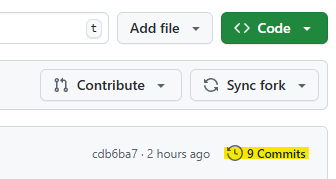
\includegraphics[scale=0.5]{../../media/github_commits.png}~~~~~~~~~~~~~
\includegraphics[scale=0.5]{../../media/github_pullrequest.png}

\end{frame}

% ======== Anaconda environments =========

\begin{frame}
\frametitle{Anaconda and Virtual Environments}
\begin{itemize}
	\item There are a lot of Python packages, and you will have multiple projects
	
	\item Project A requires \texttt{CoolPackage} v0.8 or higher; Project B requires v0.7 or lower
	
	\item <2->Not a problem! \texttt{conda} can manage virtual Python environments
	
	\item <2->Can have multiple collections/configurations of packages on your computer
	
	\item <2->Manage each separately, switch between them with a single command
	
	\item <3->We probably won't use this much, but will install more packages
	
	\item <3->Open up Anaconda Prompt (from Windows start menu, e.g.); terminal will open
\end{itemize}
\end{frame}

% ======== Installing HARK (example) =========

\begin{frame}
\frametitle{Installing New Packages}
\begin{itemize}
	\item Example: installing \texttt{HARK}, Econ-ARK's primary software package
	
	\item In Anaconda prompt, type \texttt{pip install econ-ark}, accept
	
	\item <2->\texttt{pip} is the most common \textbf{package manager}, draws on Python Package Index
	
	\item <2->\texttt{conda} is also a package manager, but \textbf{slightly} fussier
	
	\item <3->\texttt{HARK} is now available for use on your computer
	
	\item <3->But we won't be working with it yet
\end{itemize}
\end{frame}

% ======== Spyder and other IDEs =========

\begin{frame}
\frametitle{Actually Working with Python: Spyder}
\begin{itemize}
	\item You \textbf{can} write and edit Python code in any text editor
	
	\item And then run Python code from a command line with \texttt{python}
	
	\item <2->Using an \textbf{interactive development environment} (IDE) just make things nicer
	
	\item <2->Open up Spyder (e.g. from Windows start menu)
	
	\item <3->There are a lot of panes; I close all of them except console and editor
	
	\item <3->Can open them later from View menu, Panes option
	
	\item <4->Console pane: live Python environment, can run code commands one by one
	
	\item <4->Editor pane: file editor; write scripts / programs, run with green arrow in toolbar
\end{itemize}
\end{frame}

\begin{frame}
\frametitle{How to Learn Python}
\begin{itemize}
	\item We will give you hands-on instruction with Python, don't worry
	
	\item If you want to learn on your own, I recommend Kevin Sheppard's notes
	
	\item There's a copy in \texttt{/materials/setup/KevinSheppardPython.pdf}
	
	\item It's from four years ago; current Python versions are 3.10 to 3.13
	
	\item <2->Recommended reading order: Ch 1, 2, 4, 9, 10, 12, 18, 3, 6, 7, 5, 11, 15, 29
	
	\item <2->Data operations: Ch 8, 16, 14, 17, 23
	
	\item <2->More math stuff: Ch 19, 20, 21, 22
	
	\item <2->General coding: Ch 13, 24, 25, 26, 28
\end{itemize}

\end{frame}

% ======== Jupyter notebooks =========

\begin{frame}
\frametitle{Introduction to Jupyter Notebooks}
\begin{itemize}
	\item Communicating scientific ideas is sometimes aided by reader interaction
	
	\item \textbf{Jupyter notebooks} provide a way to integrate text, math, and code
	
	\item <2->Go to \texttt{https://github.com/econ-ark/HARK} and fork our repo
	
	\item <2->Then clone it to your personal computer
	
	\item <3->In Anaconda prompt, type \texttt{jupyter notebook}
	
	\item <3->Navigate to your HARK clone directory, then go to \texttt{/examples/Gentle-Intro/}
	
	\item <3->Open \texttt{Gentle-Intro-To-HARK.ipynb}
	
	\item <4->Cells can be run individually with Shift+Enter
\end{itemize}
\end{frame}

\end{document}
